\documentclass[12pt]{article}
\usepackage[utf8]{inputenc}
\usepackage{tgbonum}
\usepackage[a4paper, total={7in, 10in}]{geometry}
\usepackage{graphicx}
\usepackage{minted}
\title{Lab Assignment 5b}
\author{Akshat Mittal - 20107}
\date{June 2021}
\begin{document}
\maketitle
\vspace{7mm}
\textbf{Contents}
\vspace{7mm}
\begin{enumerate}
    \item Linear Search in array
    \item Rolling a dice 36000 times
    \item Array Grades and its operations
    \item Sum of two matrices
    \item Transpose of a matrix
    \item Product of two matrices
    \item Matrix with element -1,0,1
\end{enumerate}

\newpage
\section{}
\subsection{Code}
\inputminted{c}{q1.c}
\subsection{Output}
\begin{figure}[h]
    \centering
    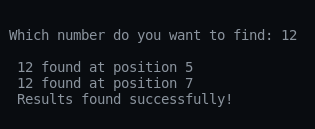
\includegraphics{1.png}
\end{figure}

\newpage
\section{}
\subsection{Code}
\inputminted{c}{q2.c}
\subsection{Output}
\begin{figure}[h]
    \centering
    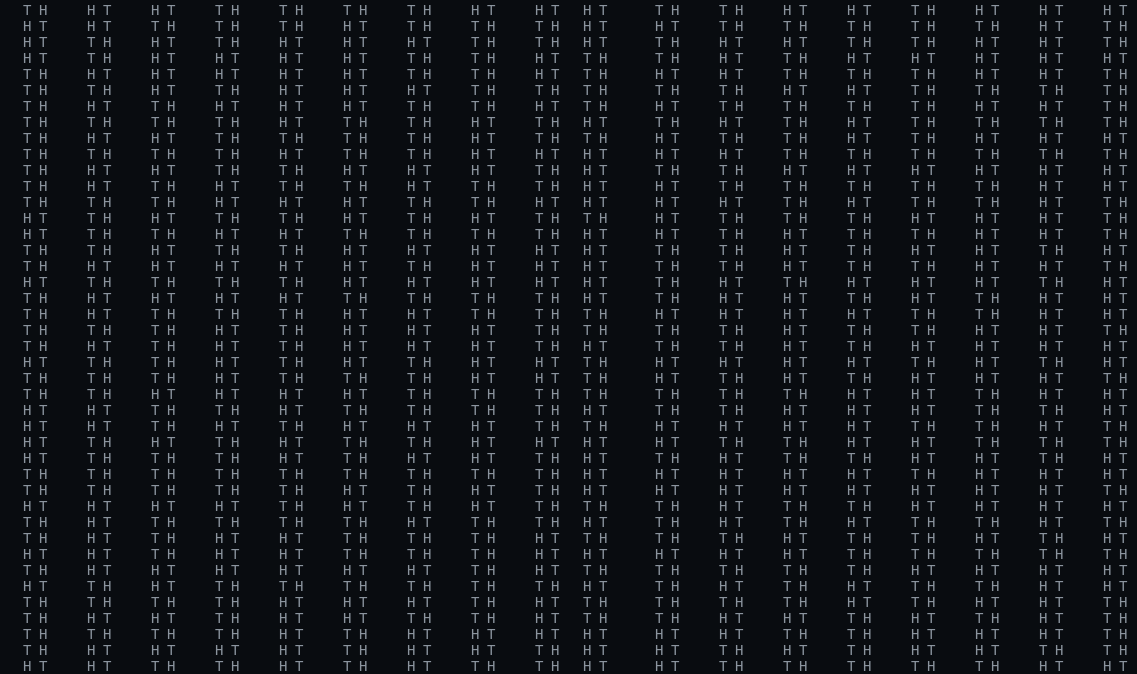
\includegraphics[width=0.76\textwidth]{2.png}
\end{figure}

\newpage
\section{}
\subsection{Code}
\inputminted{c}{q3.c}
\subsection{Output}
\begin{figure}[h]
    \centering
    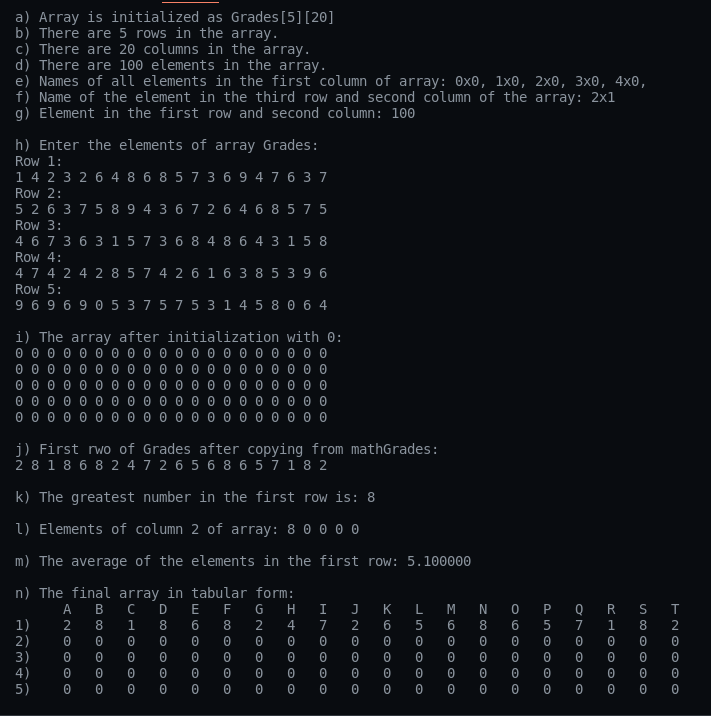
\includegraphics[width=1\textwidth]{3.png}
\end{figure}

\newpage
\section{}
\subsection{Code}
\inputminted{c}{q4.c}
\subsection{Output}
\begin{figure}[h]
    \centering
    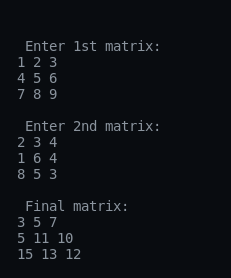
\includegraphics[width=0.35\textwidth]{4.png}
\end{figure}

\newpage
\section{}
\subsection{Code}
\inputminted{c}{q5.c}
\subsection{Output}
\begin{figure}[h]
    \centering
    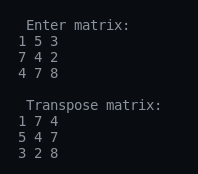
\includegraphics[width=0.4\textwidth]{5.png}
\end{figure}

\newpage
\section{}
\subsection{Code}
\inputminted{c}{q6.c}
\newpage
\subsection{Output}
\begin{figure}[h]
    \centering
    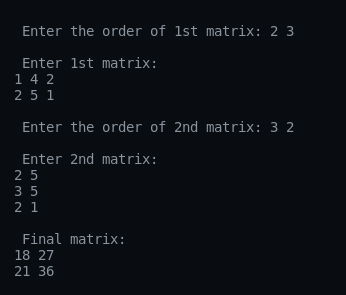
\includegraphics[width=0.75\textwidth]{6.png}
\end{figure}

\newpage
\section{}
\subsection{Code}
\inputminted{c}{q7.c}
\subsection{Output}
\begin{figure}[h]
    \centering
    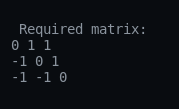
\includegraphics[width=0.5\textwidth]{7.png}
\end{figure}

\end{document}